%!TeX program=xelatex
\documentclass[a4paper]{article}

\usepackage{amsmath}
\usepackage{amssymb}
\usepackage[margin=1in]{geometry}
\usepackage{algorithm2e}
\usepackage{hyperref}
\usepackage{graphicx}
\usepackage{subcaption}

\usepackage{fontspec}
\setmainfont[Ligatures=TeX]{Palatino Linotype}

\begin{document}
    \title{Problem Outline}
    \author{Matthew Alger \\ \emph{The Australian National University}}
    \maketitle

    This document is a quick run-down on the cross-identification problem as I see it.

    As input, we have two images, one in infrared and one in radio:

    \begin{figure}[!ht]
        \centering
        \begin{subfigure}{0.3\textwidth}
            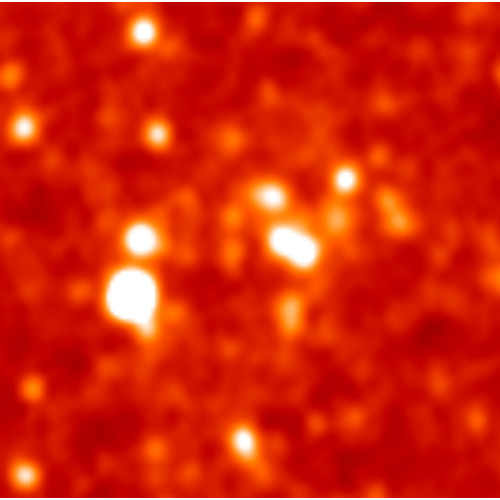
\includegraphics[width=\linewidth]{images/ARG000180p_ir.jpg}
        \end{subfigure}\quad
        \begin{subfigure}{0.3\textwidth}
            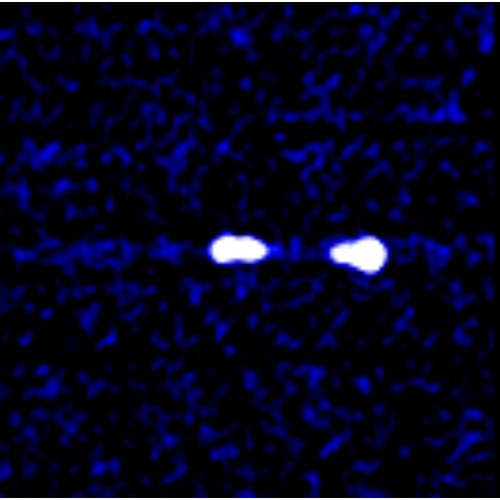
\includegraphics[width=\linewidth]{images/ARG000180p_radio.jpg}
        \end{subfigure}
    \end{figure}

    We also have some metadata associated with the subject --- mainly its location.

    From this input, we want to find the location of the radio source that emitted the jets observed in the radio image. For my project, we want to learn how to automatically perform this task using data from the Radio Galaxy Zoo.

    To learn how to perform this task, we need to break it down into a machine learning problem. First, I make the assumption that the radio sources are always located in an infrared source (i.e. a galaxy). Then, from the infrared image, we find the coordinates of all of the infrared sources. This can be possibly be done in a few ways, such as
    \begin{itemize}
        \item Finding brightness local maxima in the IR image
        \item Fitting Gaussians to the IR image
        \item Looking up the location of the subject in an infrared source catalogue
    \end{itemize}
    I'm not sure what the best approach is here, but fitting Gaussians is better than finding local maxima.

    \begin{figure}[!ht]
        \centering
        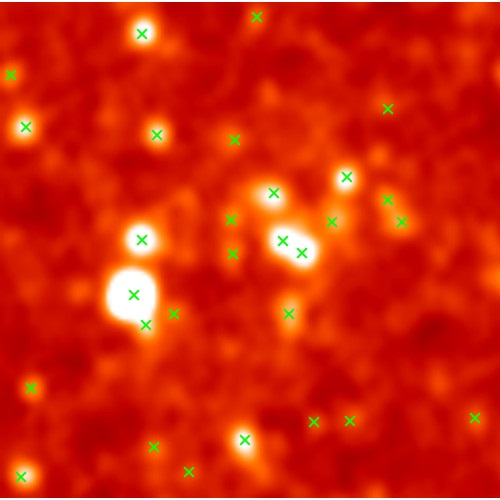
\includegraphics[width=0.3\linewidth]{images/ARG000180p_ir_potential_hosts.jpg}
    \end{figure}

    For each potential radio source location, we want to find some set of features that represents the location in some meaningful way. The way I'm going about this is to extract features from the \emph{radio} image --- it seems that the IR image itself doesn't contain much information besides the locations, though it's possible we could explicitly re-add information like brightness or spread as features later. For each location in the IR image, we sample a region of the radio image centred on the location.

    \begin{figure}[!ht]
        \centering
        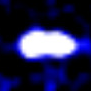
\includegraphics[width=0.15\linewidth]{images/radio_neighbourhood_1.png}\quad
        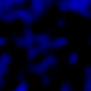
\includegraphics[width=0.15\linewidth]{images/radio_neighbourhood_2.png}\quad
        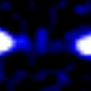
\includegraphics[width=0.15\linewidth]{images/radio_neighbourhood_3.png}
    \end{figure}

    We then run each radio image sample through an automatically-determined function to extract features. This gives us some features that represent each location.

    Then, we run the features for each location through an automatically-determined function that attempts to classify each location as ``containing the radio source'' or ``not containing the radio source''. For each location, the function will also find the probability that the classification of that location is correct. We can then choose the location with the highest probability of containing the radio source.


% \bibliographystyle{plain}
% \bibliography{papers}

\end{document}
